En este trabajo, nos disponemos a utlizar diferentes tecnicas de aprendizaje no supervisado para clasificar textos con ciertas caracteristicas. Los mismos consisten en descripciones de diversas companías y nuestro objetivo será lograr clasificar cada una en una categoria correspondiente. Contamos, ademas, con las verdaderas categorias de cada companía para realizar una validación de los datos.
Comenzaremos con una breve descripcion de los algoritmos para entender cual es el proposito y ejemplificaremos con casos de la vida real.

PCA:
Un problema comun en reconocimiento de patrones es la de seleccionar atributos. Es decir, tenemos un espacio de datos (de informacion sobre algun fenomeno que queremos estudiar, por ejemplo reconocimiento de mails de SPAM) y lo transformamos en un espacio de atributos, es decir por ejemplo, tenemos un dataset de mails y nos quedamos con la cantidad de aparicion de ciertas palabras solamente como atributos. Sin embargo, esta transformacion a veces se hace de manera que el data set pueda ser representado por un reducido numero de atributos "efectivos" (es decir, atributos que me aporten mucha informacion sobre el tipo de mail que es). Para ser mas especificos, supongamos que tenemos un vector x de m dimensiones, y queremos transmitirlo usando l numeros, con l < m, lo que implica que estamos comprimiendo datos. Si simplemente truncamos el vector, causamos un error equivalente a la suma de las varianzas de los elementos eliminados de x, entonces lo que nos preguntamos es: Existe una transformacion lineal T tal que el truncamiento de Tx tal que su error cuadratico medio sea minimo? A dicha transformacion es la que llamamos obtener las componentes principales de un vector. Veamos un ejemplo:

\begin{figure}[h!]
  \centering
  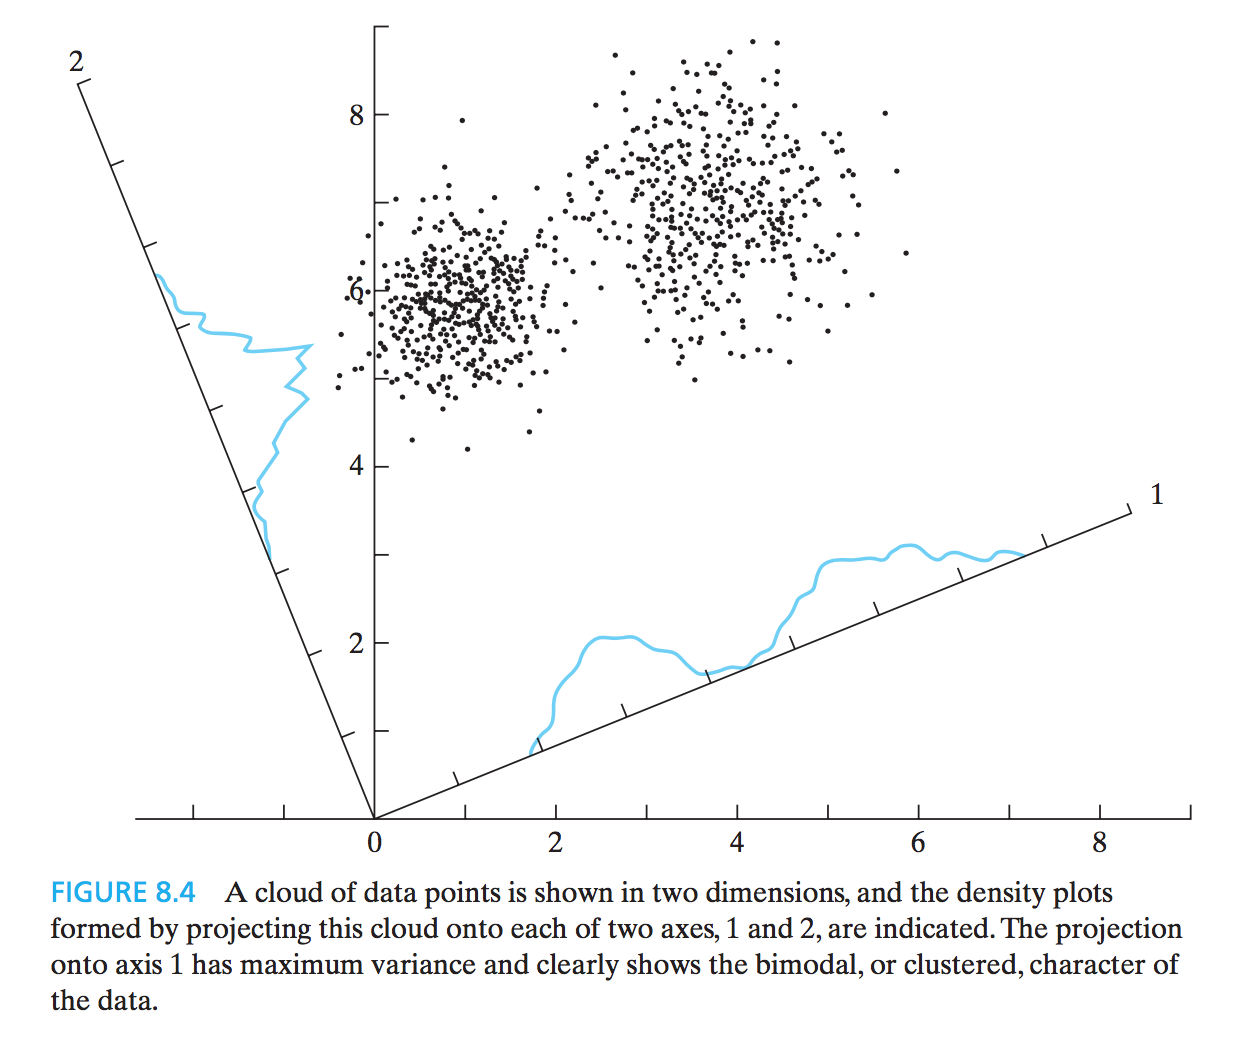
\includegraphics[width=.6\linewidth]{img/pca/dispersion}
\label{fig:test}
\end{figure}

SOM:
Es un tipo de aprendizaje no supervisado de tipo competitivo. Que queremos decir con esto? Tenemos un conjunto de neuronas de salida organizadas en una grilla de 2 dimensiones (tambien conocido como "lattice"), dichas neuronas "compiten" entre ellas para ser activadas. Pero solo una de ellas sera la que disparará (también podemos generalizarlo a grupos de neuronas, y que disparara solamente una neurona de cada grupo). Las neuronas que se activan (aquellas que ganan la competencia) las llamaremos neuronas ganadoras. Bajo esta visión lo que nosotros haremos es conocido en la literatura como winner-takes-all. Estas neuronas son inducidas a distintos estimulos (o patrones de distintas clases) para que se establezca un orden entre neuronas ganadoras. Es decir, lo que trataremos de hacer es que bajo patrones similares, vamos a querer que se activen neuronas que sean cercanas entre ellas bajo alguna metrica. En nuestra grilla podemos tomar como metrica la distancia euclediana y lo que vamos a querer respetar es que bajo un conjunto de inputs que sean muy distintos, activaciones de neuronas que esten alejadas, produciendo en nuestro mapa de neuronas "clusters" o grupos bien diferenciados de neuronas en estado exitatorio. Es decir, preservamos una topologia, a entradas de distintas clases le corresponden neuronas de distintos grupos, y cuanto mas disimilares sean estas entradas, mas lejanas seran las neuronas activadas. La motivacion de esto fue que por ejemplo, el sistema tactil (Kaas et cl., 1983), visual (Hubel and Wiesel, 1962, 1977) y acustico (Suga, 1985) son "mapeados" a diferentes areas en la corteza cerebral respetando un orden topologico.
Los mapas computacionales ofrecen cuatro propiedades importantes (Knudsen et a., 1987; Durbin and Michison, 1990).
\begin{enumerate}
\item En cada mapa, la neuronas actuan en paralelo y procesan pedazos de informacion que son similares en su naturaleza, pero proceden de diferentes reginoes en el espacio de entrada sensorial.
\item En cada etapa de la representación, cada pieza de entrada de información se mantiene en su contexto.
\item Las neuronas que tratan con inputs cercanos (parecidos) son cercanas entre ellas por lo que interactuan a travez de conexiones sinapticas cortas.
\item Los mapas contextuales pueden ser entendidos en terminos de mapas de reduccion de una dimension alta.
\end{enumerate}

Veamos una posible implementación de nuestra grilla dado un input:

\begin{figure}[h!]
  \centering
  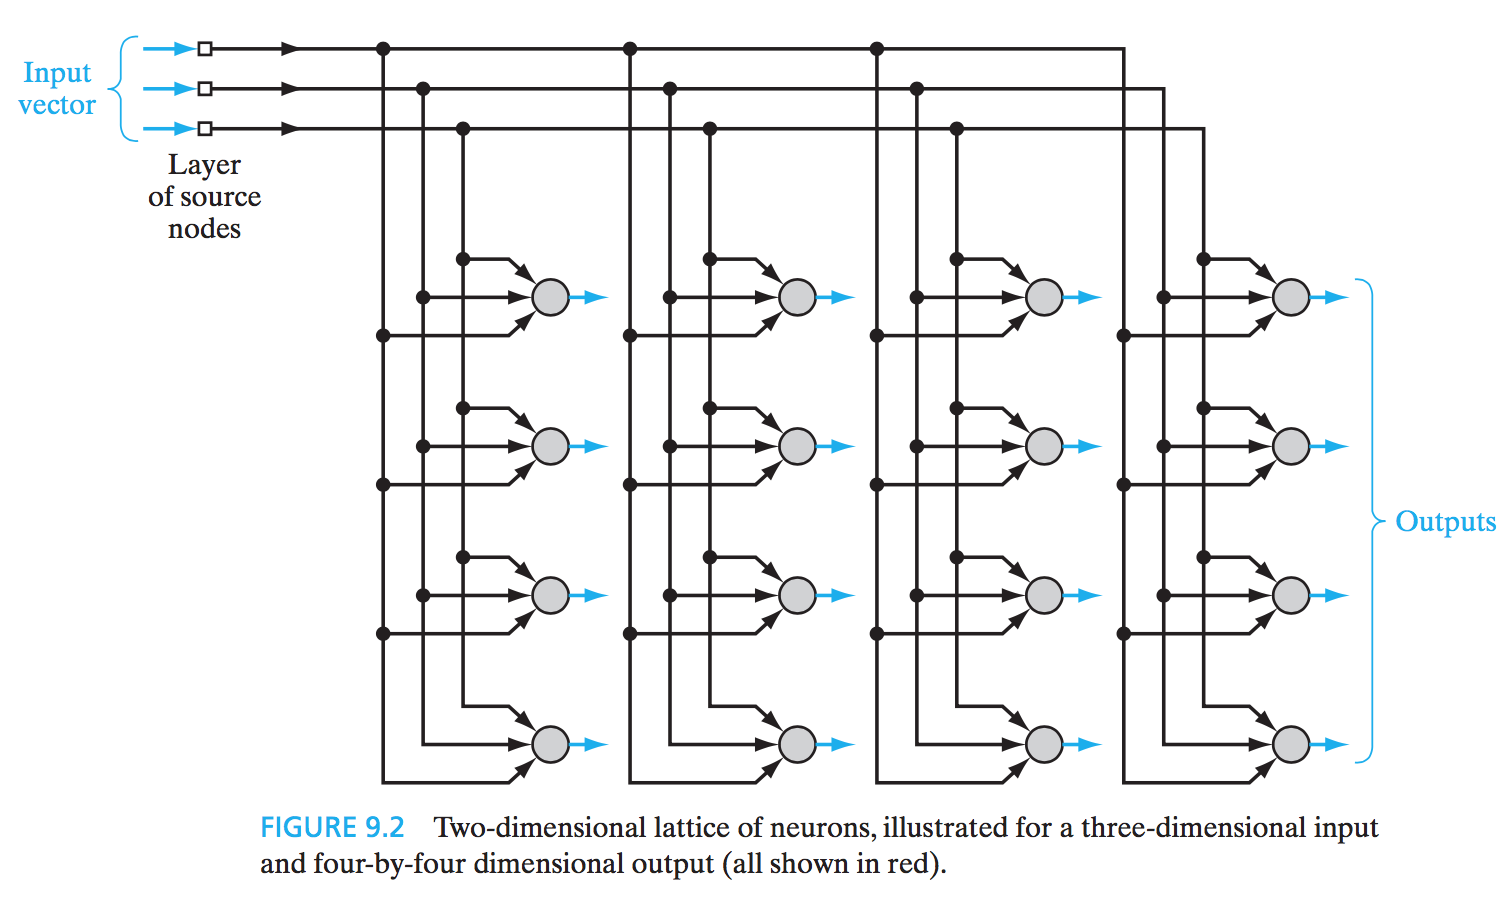
\includegraphics[width=.6\linewidth]{img/som/implementacion}
\label{fig:test}
\end{figure}

\pagebreak
Hay dos modelos implementativos para este tipo de mapas. Uno es el de Willshaw-von der Malsburg y el segundo el de Kohonen. En particular nos especializaremos en el segundo pero vamos a dar una breve reseña de cada uno.

\begin{figure}[h!]
  \centering
  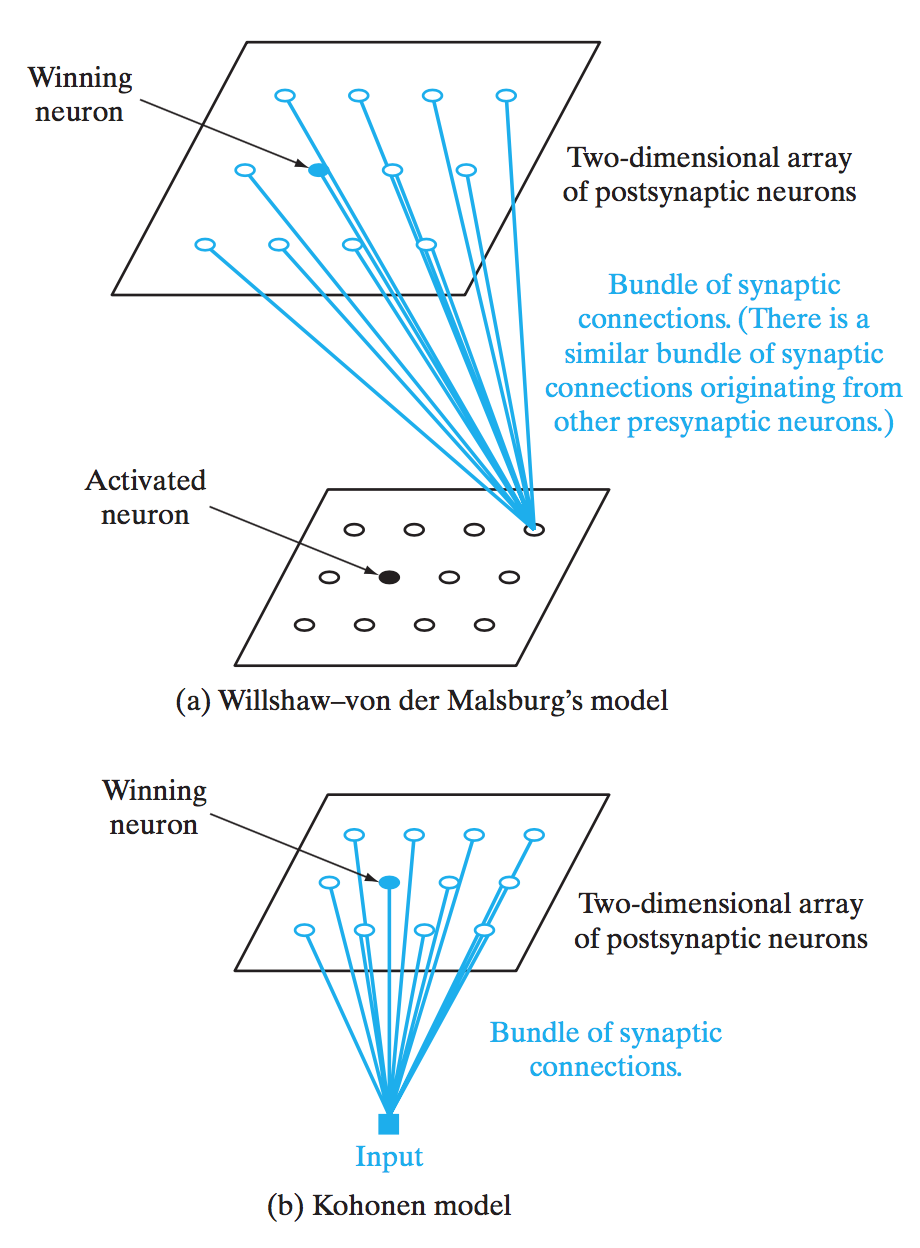
\includegraphics[width=.6\linewidth]{img/som/modelos}
\label{fig:test}
\end{figure}


El primero lo que hace es que tanto la entrada como la salida tienen la misma dimension. Es decir que si estamos usando un mapa de 2 dimensiones como salida, vamos a tratar la entrada como una grilla de neuronas de 2 dimensiones. Para entenderlo mejor, a continuacion un grafico.


Algo a remarcar es que en este modelo las neuronas postsinapticas no son del tipo winner-takes-all sino que se utiliza un threshold para asegurar que solo unas pocas son activadas. Ademas, cada uno de los pesos tiene una cota superior establecida para que no se supere y lleve a inestabilidades de la red. Su motivacion fue el mapeo de la retina a la corteza visual (se comportaban como dos grillas, por una parte tenemos a la retina que la podemos pensar como una grilla captando cada celda una porcion de luz, y esta viaja a traves de conexiones sinapticas a otra grilla que es la corteza visual, activando diferentes neuronas ante distintos patrones).



El segundo modelo no trata de explicar detalllles neurobiologicos. Lo que hacemos aqui, es capturar un vector de entrada de cualquier dimension y transformarlo a una matriz de 2 dimensiones. Es decir, es un algoritmo del tipo de vector-coding. Puede ser visto de dos maneras, una de ellas es la idea de auto organizacion, motivada por hechos neurobiologicos, y la otra es tratarlo como un codificador-decodificador cuya motivacion provino del area de teoria de las comunicaciones (Luttrell, 1989, 1991)

\begin{figure}[h!]
  \centering
  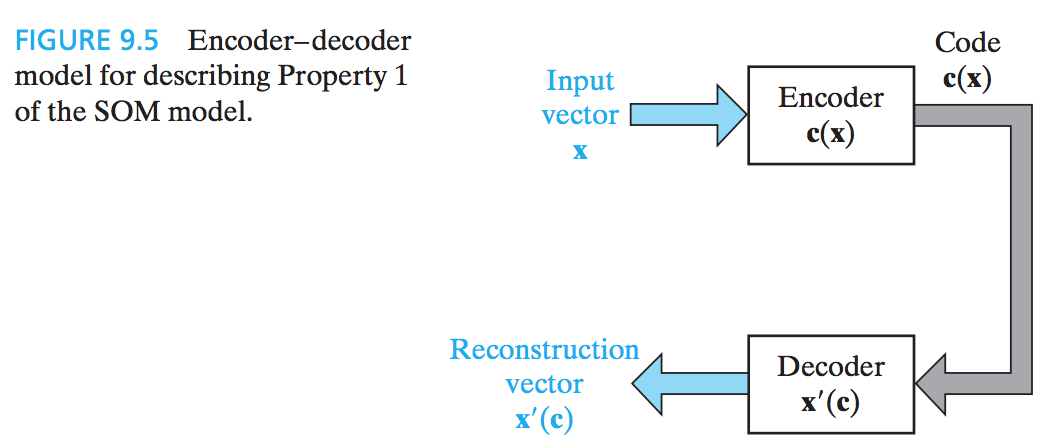
\includegraphics[width=.6\linewidth]{img/som/compresion}
\label{fig:test}
\end{figure}